
\chapter{Fundamentals of cartography and geodesy}

Since GIS inherits concepts and ideas previously used to create printed maps, it is mandatory to know them in order to correctly use the tools included in a GIS. The fundamental concepts from cartography and geodesy are the most important ones. Without them, it is not possible to understand GIS.


\section{Basic concepts of geodesy}
\pagestyle{fancy}

The main property of georeferenced information is that it has a \textbf{location}, and more particularly, a location on the earth. This location is given with \textbf{coordinates} that define it, and that requires a reference system to refer those coordinates to.

\textbf{Geodesy} is the science that provides the theoretical framework for this, and it studies the \textbf{Earth's shape}. Geodesy, through its different branches, provides methods and concepts that allow defining and using precise and rigurous coordinates to locate elements and phenomena that take place on earth.

Geodesy is needed due to the fact that the Earth is not flat, and when the area that is studied is large enough, the effect of the Earth's curvature cannot be ignored. We find that case when working with a GIS, and for this reason, GIS implement the required elements to manage geographical information taking into account the ideas and principles of geodesy.

One of the main purposes of geodesy is to establish a reference system and define a set of points (known as \textbf{geodesic vertices}), whose position is know with a high level of accuracy. Based on those points, which form a \textbf{geodesic network}, coordinates for any point on the earth surface can be computed.

\subsection{Reference surfaces}

To accomplish this, geodesy defines two basic reference surfaces: \textbf{reference ellipsoid} and \textbf{geoid}.

Earth has an spherical shape. However, it is not a perfect sphere, but instead what is called an \textbf{ellipsoid}. In an ellipsoid, the radius is not constant, and depends on the location over its surface. Using an ellipsoid to define the Earth's shape is more precise than assuming it has a spherical shape, and is needed to create accurate cartography, especially when the represented surface is not too large.

The ellipsoid provides a theoretical expression of the Earth's shape, and the next step is to determine the parameters that define it. In the case of a sphere, the only parameter needed is the radius. In the case of an ellipsoid, two parameters have to be determined: the length of semi-major and semi-minor axis.

For historical reasons, meny ellipsoids exist, all of them derived from the work of geodesist in different times and places. The first general ellipsoids, which can be used for representing any place on Earth's surface, appeared aproximately a hundred years ago, created with the purpose of having an international reference that can be used for creating cartography in different areas of our planet. The \textbf{WGS--84} ellipsoid is one of the most populars nowadays, and it is use by the GPS positioning system. 


The other reference surface is the geoid, defined as the three-dimensional surface where every point have the same gravitational attraction. It is an equipotential surface that results from assuming average ocean levels and extending them under the Earth's surface.

As in the case of ellipsoids, there are several geoids as well. These are not constant, and evolve to adapt to the changes that take place on the Earth's surface.

Figure  \ref{Fig:Three_surfaces} shows a comparison of the three surfaces: Earth's surface, geoid and ellipsoid.

\begin{figure}
\centering
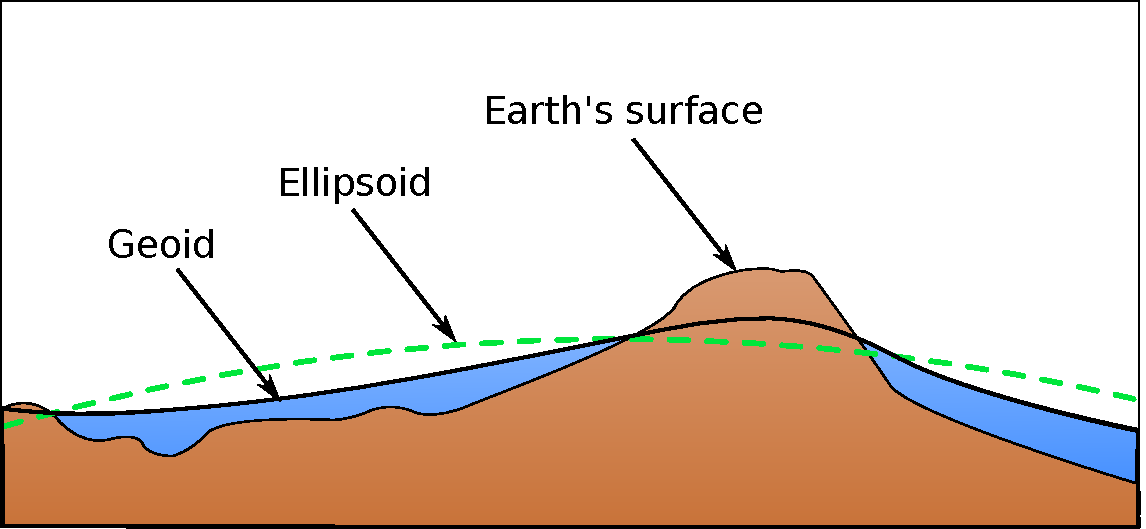
\includegraphics[width=.7\columnwidth]{Cartography/Three_surfaces.pdf}
\caption{\small Comparison of the three fundamental surfaces: Earth's surface, geoid and ellipsoid.(Adapted from Wikipedia).}
\label{Fig:Three_surfaces} 
\end{figure}

In a \textbf{general ellipsoid}, both the location of it center of gravity and it equatorial plane match those of the Earth. In a \textbf{local ellipsoid}, this does not have to be true, and the ellipsoid by itself is not enough, since we do not know how to place it relative to the real Earh's surface.

The concept of \textbf{datum} solves this problem. A \textbf{datum} is the combination of a reference surface (the ellipsoid) and a point in which it is linked to the geoid. That point is called the \textbf{fundamental point}, and the ellipsoid is tangent to the geoid there. At the fundamental point, a line perpendicular to the geoid is identical to a line perpendicular to the ellipsoid. 

\subsection{Coordinate reference systems}

Once we have a model to define the Earth's shape, we can establish a system to code any position over its surface and asign a corresponding coordinate to it. The combination of a coordinate system and a datum is called a \textbf{coordinate reference system} (CRS).

Regarding the coordinate system, we have two main alternatives: using the elements of \textbf{spherical geometry} using the concepts of \textbf{plane geometry}. In this last case, we need a \textbf{projection system} to place the elements on the surface of the ellipsoid into a plane.

\textbf{Geographical coordinates} use a spherical coordinates syste in which the location of every point is defined by two angular values: \textbf{latitude} and \textbf{longitude}. Lines of equal latitude are called \textbf{parallels}, while lines of equal longitud are called \textbf{meridians}.

Geographical coordinates are of great utility, especially when working with large regions. However, it is not a cartesian system, and \textbf{it is difficult to perform tasks such as measuring distances or areas}. To simplify operations like those ones, we need cartesian coordinates. To assign a plane coordinate to every point on te Earth's surface (which is not a plane), we must use a \textbf{cartographic projection}.

Earth's surface is not \textbf{developable}. That is, it cannot be flattened without distortion. For this reason, we need a methodology for converting points on this surface into points on a plane. Figure \ref{Fig:Projection} shows this idea.

\begin{figure}
\centering
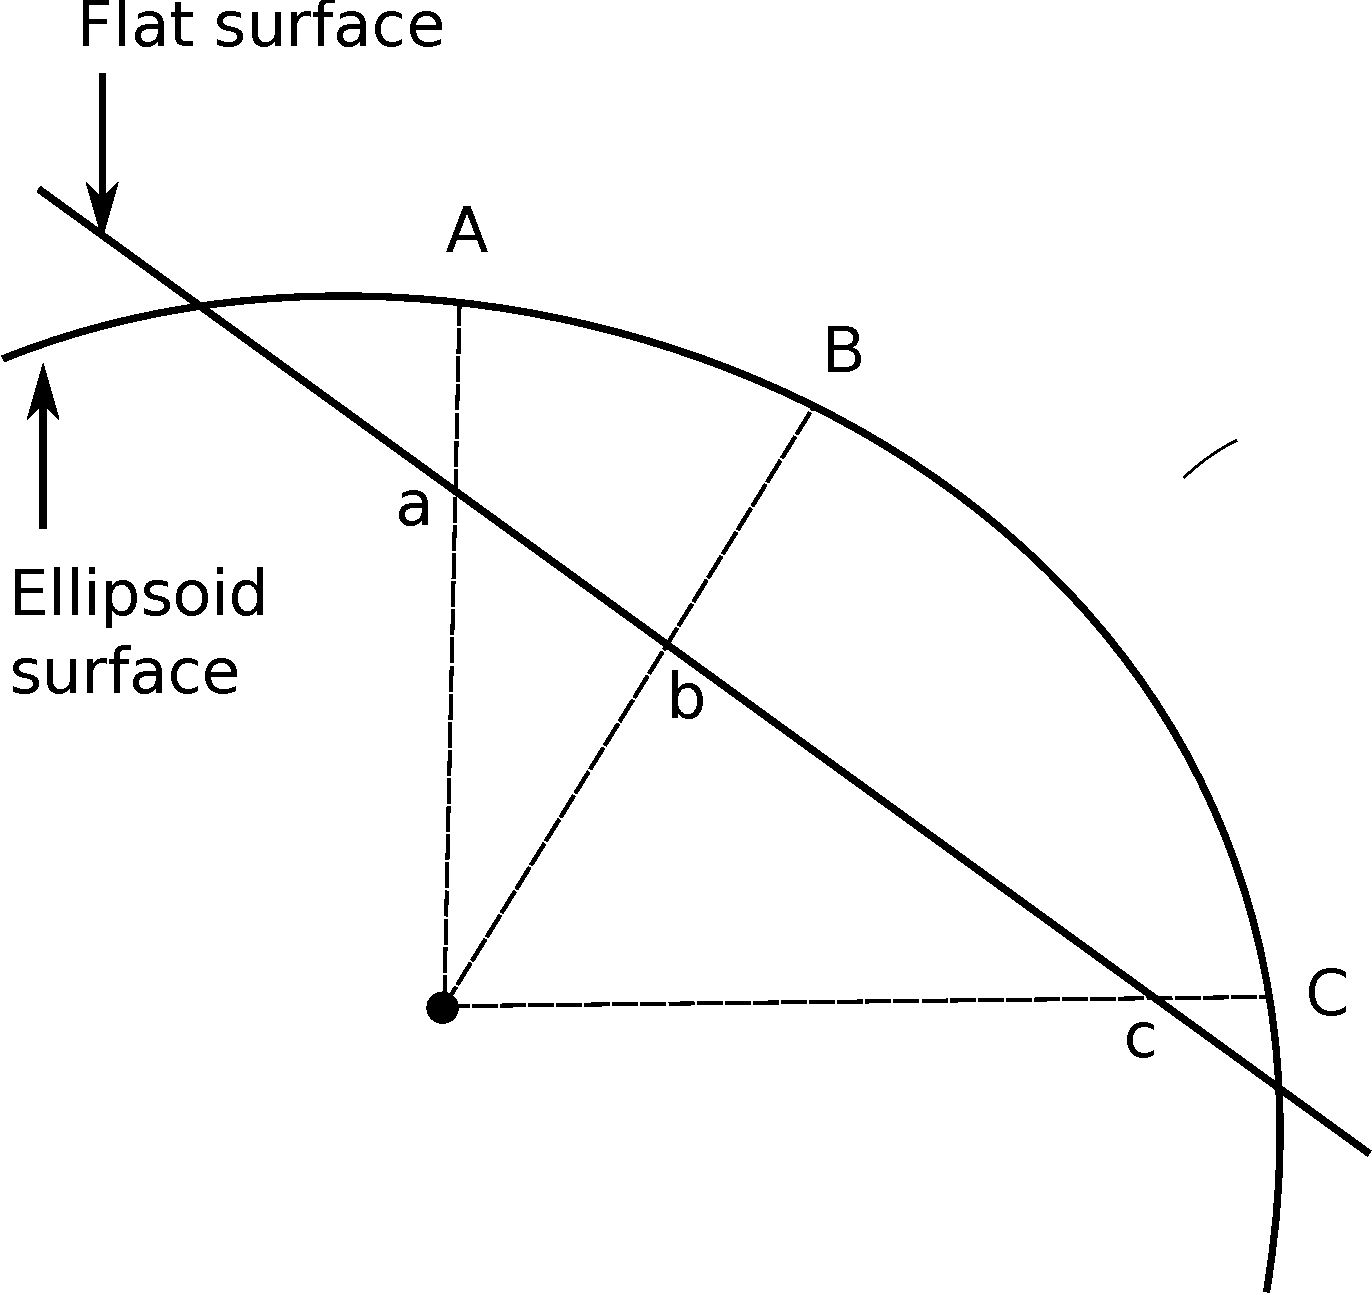
\includegraphics[width=.5\columnwidth]{Cartography/Projection.pdf}
\caption{\small Graphical explanation of a projection. Points $A, B$ and $C$ on the surface of the ellipsoid are converteed into their equivalent points $a, b$ and $c$ on a plane.}
\label{Fig:Projection} 
\end{figure}

In the case depicted in the figure, point are projected directly onto the plane. Another alternative is to project them onto a surface that, unlike the surface defined by a sphere or an ellipsoid, can be developed (that is, it can be flattened later without distortion). The most usual surfaces for that are the cylinder and the cone. The corresponding projections are called \textbf{conical projections} and \textbf{cylindrical projections}.

It can be seen in the figure that projecting points introduces distortions. For instance, the distance between points $A$ and $B$ is not the same as the distance between points $a$ and $b$. All projections introduce some sort of distorsion, regardless of their properties. Depending on the metric properties that are preserved undistorted, we have \textbf{equal-area projections} (which preserve area), \textbf{conformal} (preserve angles and shapes) o \textbf{equidistant} (preserve distances).

Depending on the context and the purpose of our data, we might use one or another type of projection. 

One of the most widespread projections nowadays is the \textbf{Universal Transverse Mercator}, which is the basis for the \textbf{UTM coordinate system}. This system is not just a projection, but a complete system of many of them. Earth's surface is divided in rectangular regions, and for each of them a different projection an a different set of geodetical parameters are used. It uses a single ellipsoid: WGS-84.

In the UTM system, coordinate are not expressed as absolute coordinates, but instead the are refered to the corresponding rectangle, as relatives coordinates within it.

The UTM grid contains 60 zones, each 6\degree of longitude in with. Zone 1 is locateed between 180\degree y 174\degree West, and numbering increases eastward.

Each zone is segmented into 20 latitude bands, ranging from 80\degree South to 84\degree North. These are coded with letters from C to X, excluding I and O due to their similarity to the numerals one and zero. Each band has 8\degree of latitude in height, except the X band, which has 12. 

A UTM rectangle is therefore defined by \textbf{a number and a letter}, and the coordinates that are used to locate a given point on the Earth's surface are referred to the zone it belongs to. Coordinates are expressed in meters and represent the distance between the point and the origin of the UTM rectangle. The origin is located at the intersection between  the meridian passing through the center of the zone and the equator.

To avoid negative numbers, the origin is assumed to have and X coordinate of 500000 meters and a Y coordinate of 10000000 meters, causing all coordinates referred to it to have only positive values.

\subsection{Coordinate conversion and transformation}

It is common when working with a GIS to have layers in \textbf{several different coordinate systems}, or in the same coordinate system but using different parameters (such as for instance, a different datum). In order to use be able to use those layers together, we have to work in a single coordinate systems, and at least some of those layers will have to be converted to it. That is known as \textbf{coordinate conversion}. If the origin and destination coordinate systems have a different datum, coordinate conversion is called \textbf{coordinate transformation}.


In a GIS, conversion and transformation capabilities allow to generate new layers that use a different CRS. Also, GIS include the ability to perform them \emph{on-the-fly} when layers are rendered, so we can create a map with layers that do not share the same CRS. These are correctly represented on the map and ``match'' one with another, since the GIS is automatically performing the corresponding changes to their coordinates to have them in a common CRS.

To facilitate the use of coordinate reference systems, there are initiatives that try organize and code them, so each system can be easily identified by a unique code. The most common coding system are the \textbf{EPSG} codes defined by the International Association of Oil and Gas Producers. 


\section{Basic cartographic concepts}

Among the fundamental concepts of cartography that any GIS user has to know, \textbf{scale} is the most important one. The scale of a map represent the \textbf{size ratio} between the ``map'' that would be obtained by developing the real surface we are representing (the Earth's surface in this case), and the scale of our smaller map. Knowing this ratio, we can know the real measures of the elements that are included in the map, since we can convert the measurements that we make on it into real-world measures. It's important to keep in mid that these measures are not so ``real'', since the projection might have distorted them, but they are, nonetheless, measures at the original scale of the object that is measured.

Scale is usually expressed as a quotient between the distance measured in a map and the distance that this measure represents in reality. For instance, a 1:50000 scale means that 1 centimeter in a map is equivalent to 50000 centimeters in reality, that is 500 meters. This value is known as the \textbf{numeric scale}.

Regardless of the projection used, scale is completely true only at certain points in the map. In the rest of them scale changes. The relation between the scale in those points and the numeric scales is known as the \textbf{scale factor}.

Although scale is traditionally understood as a concept related to the data representation, geographical data has an inherent scale not related to its representation, but to the level of detail with which the data was captured on the field. It's more correct to understand scale as something related to the data \textbf{resolution}, that is, related to the \textbf{minimum mapped size}.

The resolution of the human eye is 0.2mm. With that value, and the scale we want to use for a map, we can know the level of detail that we need to use when capturing data to be used as part of that map. 

In a GIS, as we have seen, data does not contain its visualization. That means that we can visualize it at any scale (and that is very easy to do with the zoom tools that are found in most GIS software). However, data has been captured at a given level of detail, However, data has been captured at a given level of detail, which defines the scale meant to be used and represents a limitation of that data. It will not be correct to represent it beyond that scale. In other words, to create a map at a more detailed scale, we will need more detailed data. It's easy to forget that when using a GIS.

Raster layers, as we have seen, have a \textbf{cell size}, which defines the resolution of the layer and is related to scale.

Related to the concept of scale, we find the so-called \textbf{cartographic generalization}. To generalize means to express an idea or information in a more succint manner, so it can be more useful in a given context. In a GIS, generalization is needed to represent data at a smaller (less detailed) scale that its inherent one, mainly because of the limitiations imposed by rendering devices. For instance if we have a layer with the roads of a given country, it makes no sense to use it in a map that represents the whole planet. We will get a mass of lines, and whoever uses that map will not be able to differentiate between them. Also, rendering all those lines will consume a lot of processing power. A much more interesting option would be to just take that main highways and motorways, and to not paint the rest of them. The map will be clearer and more useful, and the screen rendering will be much faster.

\begin{figure}[!hbt]
\centering
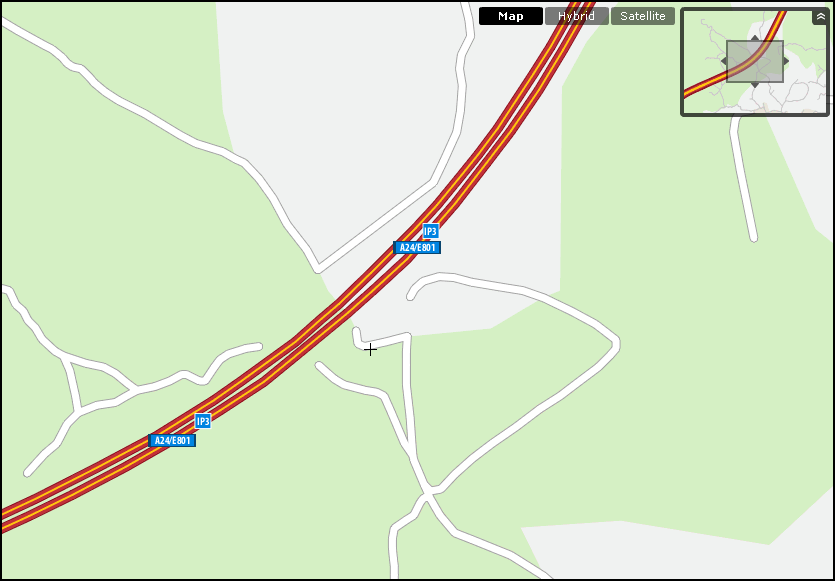
\includegraphics[width=.75\columnwidth]{Cartography/Generalization_aggregation.png}
\caption{\small Generalization by aggregation. Two roads that are almost paralell are represented as two separate elements in the map, but in the overview map of the upper-left corner, with a smaller level of detail, they are generalized as one single element. (Taken from Yahoo Maps.)}
\label{Fig:Generalization_aggregation} 
\end{figure}


Generalization in the context of a GIS also includes other changes that are made to improve the quality of the map and improve the way it conveys its information. This might not imply reducing the level of detail, but just altering the data for purely cartographic purposes.

For instance, if we are representing that road layer in a map that covers the entire world, we should not paint the roads at their real size. They would be too thin and almost invisible. We will paint them much thicker, thus creating a map that might be less correct (we are distorting the real size of those layer), but is much more useful.

Generalization is, therefore, a process whose main purpose is \textbf{to produce a cartographic image more legible and expressive}, selecting and adjusting the elements contained in a the map. It emphasizes the important ones, while it ommits the least important ones.

Some of the most relevant operations in cartographic generalization are \textbf{simplification} (representing an element that is less complex), \textbf{aggregation} (representing several elements as just one ---Figure \ref{Fig:Generalization_aggregation}---), \textbf{exaggeration} (representing elements with a larger size) and \textbf{displacement} (representing elements at a different location, to ensure legibility).


In a GIS, generalization can be implemented as part of the visualization mechanism. That is, when rendering a layer, it is modified at that same momento according to the cartographic scale and other factors. This is a time consuming procedure, and it usually does not yield good results, mainly because of the complexity of the process, which is hard to automate.

\begin{figure}[!hbt]
\centering
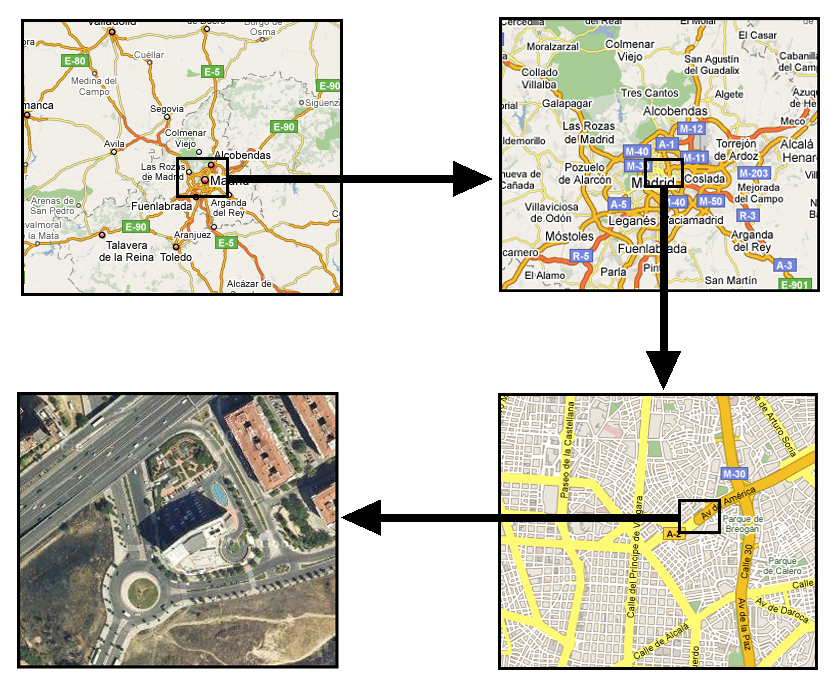
\includegraphics[width=\textwidth]{Cartography/GIS_multi_scale.png}
\caption{\small In a GIS, it is common to use information at different scales. The current cartographic scale will define which part of it rendered and which one is not.}
\label{Fig:GIS_multi_scale} 
\end{figure}

An alternative solution is to use a multi-scale approach (Figure \ref{Fig:GIS_multi_scale}). Information for a given study area is prepared at differnt scales (using generalization based on a single one or just using layers with a different origin), and the most convenient one is used in each case depending on the current scale. This is the equivalent of having several printed maps at different scales.

The concept of \textbf{layer}, which we will see in the next chapter, is key for this multi-scale approach.

In the case of images, this approach implies creating the so-called \textbf{pyramids}. Instead of using a single image, we have a set of them with different cell sizes. To optimize data handling and minimize the amount of data to be processed when rendering the image, the layerin the pyramid that best fits the current scale is used.

\pagestyle{empty}
